\documentclass[border=10pt]{standalone}
\usepackage[svgnames]{xcolor}
\usepackage{amsmath}
\usepackage{pgfplots}
\pgfplotsset{compat=newest}
\usepackage[sfdefault]{FiraSans}
\usepackage{FiraMono}
\renewcommand*\familydefault{\sfdefault}
\begin{document}
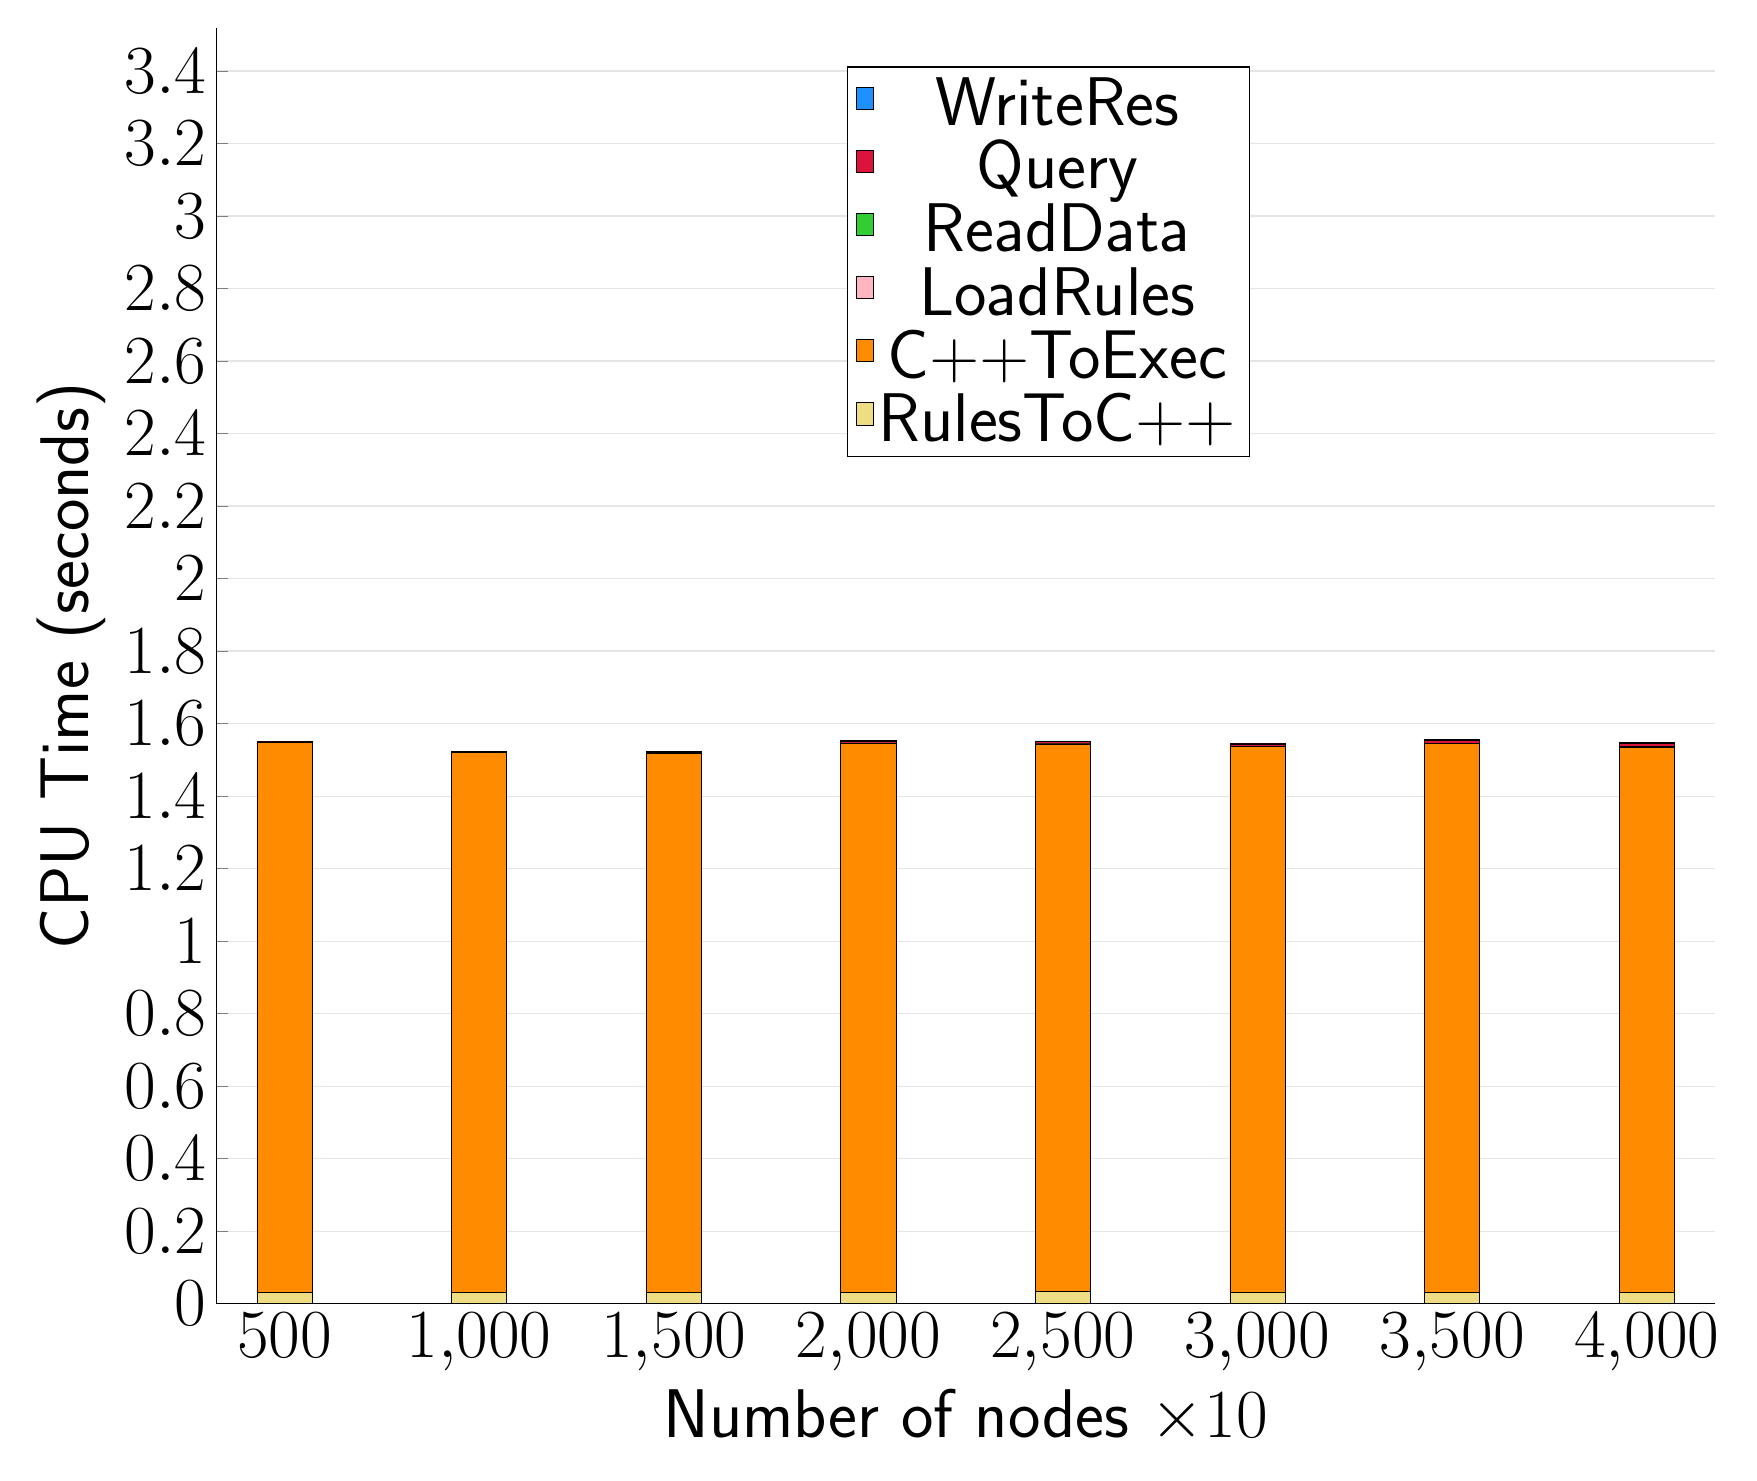
\begin{tikzpicture}
\begin{axis}[
   ybar stacked,
   width=1.7\textwidth,
   bar width=0.7cm,
   ymajorgrids, tick align=inside,
   major grid style={draw=gray!20},
   xtick=data,
   ymin=0, ymax=3.518,
   axis x line*=bottom,
   axis y line*=left,
   enlarge x limits=0.05,
   legend style={
       at={(0.69, 0.97)},
       anchor=north east,
       legend columns=1,
       font=\Huge,
   },
   ylabel={CPU Time (seconds)},
   xlabel={Number of nodes $\times 10$},
   label style={font=\Huge},
   tick label style={font=\Huge},
]
\addlegendimage{fill=DodgerBlue, draw=black, line width=0.2pt}
\addlegendentry{WriteRes}
\addlegendimage{fill=Crimson, draw=black, line width=0.2pt}
\addlegendentry{Query}
\addlegendimage{fill=LimeGreen, draw=black, line width=0.2pt}
\addlegendentry{ReadData}
\addlegendimage{fill=LightPink, draw=black, line width=0.2pt}
\addlegendentry{LoadRules}
\addlegendimage{fill=DarkOrange, draw=black, line width=0.2pt}
\addlegendentry{C++ToExec}
\addlegendimage{fill=LightGoldenrod, draw=black, line width=0.2pt}
\addlegendentry{RulesToC++}
\addplot +[fill=LightGoldenrod, draw=black, line width=0.2pt] coordinates {
(500, 0.030000000000000006)
(1000, 0.031000000000000007)
(1500, 0.030000000000000006)
(2000, 0.030000000000000006)
(2500, 0.033999999999999996)
(3000, 0.031000000000000007)
(3500, 0.030000000000000006)
(4000, 0.031000000000000007)
};
\addplot +[fill=DarkOrange, draw=black, line width=0.2pt] coordinates {
(500, 1.518)
(1000, 1.489)
(1500, 1.487)
(2000, 1.516)
(2500, 1.5099999999999998)
(3000, 1.5050000000000001)
(3500, 1.515)
(4000, 1.504)
};
\addplot +[fill=LightPink, draw=black, line width=0.2pt] coordinates {
(500, 0.00011949999999999999)
(1000, 0.00011960000000000001)
(1500, 0.00011150000000000001)
(2000, 0.00011889999999999999)
(2500, 0.00012269999999999997)
(3000, 0.0001098)
(3500, 0.00010529999999999998)
(4000, 0.00010920000000000001)
};
\addplot +[fill=LimeGreen, draw=black, line width=0.2pt] coordinates {
(500, 0.0003804999999999999)
(1000, 0.00048340000000000004)
(1500, 0.0006138999999999999)
(2000, 0.0006900999999999999)
(2500, 0.0007976999999999999)
(3000, 0.000911)
(3500, 0.0009507)
(4000, 0.00108)
};
\addplot +[fill=Crimson, draw=black, line width=0.2pt] coordinates {
(500, 0.0011500000000000002)
(1000, 0.0024479000000000002)
(1500, 0.0037695000000000007)
(2000, 0.004655299999999999)
(2500, 0.005810600000000001)
(3000, 0.0070704)
(3500, 0.007906199999999999)
(4000, 0.009300300000000001)
};
\addplot +[fill=DodgerBlue, draw=black, line width=0.2pt] coordinates {
(500, 0.00047829999999999997)
(1000, 0.000695)
(1500, 0.0009360999999999999)
(2000, 0.0011103)
(2500, 0.0013639999999999998)
(3000, 0.0015537)
(3500, 0.0016866000000000003)
(4000, 0.0019223)
};
\end{axis}
\end{tikzpicture}

\end{document}
